%=========================================================
\chapter{Marco Teórico}
\label{cap:MarcoTeorico}

	Actualmente, las instituciones educativas enfrentan desafíos significativos en cuanto a la protección de la identidad estudiantil y la seguridad académica, especialmente durante evaluaciones de alta importancia académica. En el Instituto Politécnico Nacional (IPN), particularmente en la Escuela Superior de Cómputo (ESCOM), los Exámenes a Título de Suficiencia (ETS) constituyen una oportunidad para que los estudiantes acrediten asignaturas pendientes. No obstante, la ausencia de mecanismos de autenticación robustos ha facilitado casos de suplantación de identidad, comprometiendo así la integridad académica y la seguridad dentro del plantel.
	
	Este proyecto propone el desarrollo de un sistema de identificación y control de acceso basado en reconocimiento facial y códigos QR, integrado en una aplicacióm móvil para dispositivos Android. La solución busca no solo prevenir la suplantación de identidad, sino también facilitar y agilizar los procesos de verificación por parte de docentes y personal de seguridad. 
	
	Para sustentar técnicamente esta propuesta, el marco teórico explora conceptos clave como los ETS, tecnologías biométricas, desarrollo de software móvil y arquitecturas de sistemas, proporcionando así una base sólida para el diseño e implementación del prototipo.
	
%---------------------------------------------------------
% !TeX root = ../ejemplo.tex

\section{Evaluaciones a Título de Suficiencia (ETS)}
En el Instituto Politécnico Nacional (IPN), incluyendo unidades académicas como la Escuela Superior de Cómputo (ESCOM), la acreditación de cada unidad de aprendizaje se realiza semestralmente a través de 3 evaluaciones ordinarias. Si un alumno no acredita alguna unidad de aprendizaje, tendrá la oportunidad de presentar una evaluación extraordinaria. Estos procedimientos están detallados en el programa de estudios y se encuentran especificados en el calendario académico.

El alumno que no logre acreditar una o más de las unidades de aprendizaje en la que se haya inscrito podrá optar por acreditarlas mediante Evaluación a Título de Suficiencia, de acuerdo con lo establecido en el Artículo 39 del Reglamento Interno del IPN, que señala: 

\begin{quote}
	``La evaluación del aprendizaje se llevará a cabo a través de exámenes ordinarios, extraordinarios y a título de suficiencia, cuyos requisitos y procedimientos de elaboración, presentación y exención, así como de otros mecanismos de evaluación continua, se realizarán en los términos que fijen los planes y programas de estudio, el presente Reglamento y los reglamentos respectivos.''
\end{quote}

Existen dos rondas de ETS:
\begin{itemize}
	\item ETS Ordinario: Esta es la primera oportunidad que tiene el alumno para acreditar la materia en la que no obtuvo una calificación aprobatoria. Los ETS ordinarios generalmente se aplican al finalizar el semestre, permitiendo al estudiante demostrar sus conocimientos sin necesidad de repetir el curso completo. 
	\item ETS Especiales: Si el alumno no acredita la materia en el ETS ordinario, puede optar por presentar un ETS Especial. Esta es la segunda oportunidad que tiene el alumno para pasar la materia. Esta evaluación adicional suele programarse el primer viernes del nuevo semestre, brindando al estudiante una opción rápida para regularizar sus situación académica y continuar avanzando en su plan de estudios. 
\end{itemize}

\subsection{Procedimiento para realizar un ETS}
\begin{itemize}
	\item Pagar en caja, verificar que estén correctos los siguientes datos: Nombre, Boleta, Carrera y Número de unidades de aprendizaje.
	\item Acudir a ventanilla de gestión escolar para generar créditos en el “SAES”.
	\item Una vez generados los créditos, inscribe las unidades de aprendizaje en la página del “SAES”.
	\item Entregar en ventanilla de gestión escolar, el comprobante de inscripción de ES generador por SAES, y el recibo de pago para dar fin a la inscripción al ETS. 
	\item  Acudir el día y la hora establecida en el calendario.
\end{itemize}
%---------------------------------------------------------
% !TeX root = ../ejemplo.tex

\section{Códigos QR}

Actualmente las credenciales del IPN incluyen un código QR que, al ser escaneado, proporcionan acceso a la información del alumno.
Este Código QR contiene datos esenciales como el nombre completo del estudiante, numero de boleta, la carrera en la que está inscrito y su fotografía. Además, en algunas unidades académicas del IPN, los códigos QR de las credenciales se utilizan como un medio de verificación de identidad para el acceso a las instalaciones mediante el uso de torniquetes electrónicos.

Para la elaboración de nuestro TT, el código QR desempeña un papel fundamental en la corroboración de la identidad de los estudiantes. Las credenciales escolares al contener un código QR se puede aprovechar la capacidad para almacenar y transmitir información de manera segura y rápida. Este enfoque nos permite verificar la información del estudiante mediante un simple escaneo, reduciendo el tiempo necesario para corroborar la identidad. Al escanear el código QR en la credencial. El sistema accede a los datos del alumno, lo cual permite verificar si coincide con la persona que se presenta al ETS.

Un código QR es un tipo de código de barras bidimensionales que solo se puede leer con teléfonos inteligentes u otros dispositivos dedicados a la lectura de estos códigos. Cuando se lee un código QR, los dispositivos se conectan directamente a mensajes de texto, correos electrónicos, sitios web, números de teléfono, etc \cite{CitaA01}.

\subsection{Anatomía de un código QR}
\title{Patrones de detección de posición}\\

\begin{figure}[htbp]
	\begin{center}
		\fbox{
\includegraphics[width=.24\textwidth]{images/img01}}
		\caption{Patrones de detección de posición \cite{CitaA01}.}
		\label{fig:Patrones de deteccion de posicion2}
	\end{center}
\end{figure}

Los patrones de detección de posición se encuentran en las tres esquinas del código. Gracias a ellos, el escáner puede reconocer y leer el código QR rápidamente. Estos marcadores indican la dirección en la que se imprimió el código QR y ayudan a su identificación y orientación. \\

\title{Patrones de alineación}

\begin{figure}[htbp]
	\begin{center}
		\fbox{
\includegraphics[width=.24\textwidth]{images/img02}}
		\caption{Patrones de alineación \cite{CitaA01}.}
		\label{fig:Patrones de alineacion1}
	\end{center}
\end{figure}

Usados para corregir la distorsión del código QR en superficies curvas. El tamaño y la cantidad de los patrones de alineación pueden variar según el volumen de la información almacenada en el código \cite{CitaA01}. \\

\title{Patrones de temporización}

\begin{figure}[htbp]
	\begin{center}
		\fbox{
\includegraphics[width=.24\textwidth]{images/img03}}
		\caption{Patrones de temporización \cite{CitaA01}.}
		\label{fig:temporizacion}
	\end{center}
\end{figure}

La alternancia de los módulos negros y blancos del código QR detrmina el sistema de información, también llamado cuadrícula de datos. Con estas líneas, el escáner reconoce la matriz de datos. 

\newpage

\title{Información sobre la versión}

\begin{figure}[htbp]
	\begin{center}
		\fbox{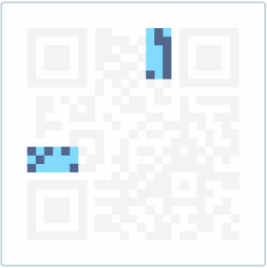
\includegraphics[width=.24\textwidth]{images/img04}}
		\caption{Información sobre la versión \cite{CitaA01}.}
		\label{fig:version}
	\end{center}
\end{figure}

Estos marcadores indican cuál de las 40 versiones del código QR está siendo usada. Normalmente las versiones utilizadas son de 1 a 7. \cite{CitaA01}\\

\title{Información del formato}

\begin{figure}[htbp]
	\begin{center}
		\fbox{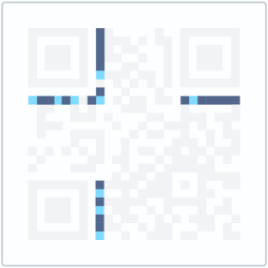
\includegraphics[width=.24\textwidth]{images/img05}}
		\caption{Información del formato \cite{CitaA01}.}
		\label{fig:formato2}
	\end{center}
\end{figure}

Contiene información sobre la tolerancia a los errores y el patrón del enmascaramiento de datos. La información sobre el formato facilita el escaneo del código. \cite{CitaA01}\\

\newpage
\title{Código de corrección de datos y errores}

\begin{figure}[htbp]
	\begin{center}
		\fbox{
\includegraphics[width=.24\textwidth]{images/img06}}
		\caption{Código de corrección de datos y errores \cite{CitaA01}.}
		\label{fig:erroresDatos}
	\end{center}
\end{figure}

El sistema de corrección de errores del código QR almacena toda la información y comparte el espacio con los módulos de corrección de errores, que permiten reconstruir los datos perdidos\cite{CitaA01} . \\

\title{Márgenes}

\begin{figure}[htbp]
	\begin{center}
		\fbox{
\includegraphics[width=.24\textwidth]{images/img07}}
		\caption{Márgenes \cite{CitaA01}}
		\label{fig:margenes}
	\end{center}
\end{figure}

Los márgenes, o también llamado zona quieta, alrededor del código QR son similares al espacio blanco en un diseño, proporcionan estructura y una mejor comprensión. Pero, ¿cómo? Para que el software de escaneo identifique bien el límite del código QR de sus alrededores, los márgenes son vitales.

\subsection{Fiabilidad de los códigos QR}
Los códigos QR están diseñados para mantener la información legible, aunque estén oscuros o dañados. Esto se logra mediante la compensación de errores, es decir, insertando la información varias veces. Con un alto nivel de seguridad, los códigos QR pueden leerse incluso si un tercio de su información es ilegible. Esto hace que los códigos QR sean muy fiables a la hora de guardar información. \\


%---------------------------------------------------------
% !TeX root = ../ejemplo.tex

\section{Desarrollo de la Aplicación Móvil}

Una aplicación móvil es un tipo de software diseñado para ejecutarse en dispositivos móviles, como teléfonos inteligentes o tabletas. A diferencia de las aplicaciones tradicionales para computadoras de escritorio, las aplicaciones móviles están optimizadas para operar con los recursos limitados de hardware de los dispositivos móviles, brindando funcionalidades específicas de manera eficiente. Aunque los dispositivos actuales son mucho más sofisticados que en sus primeras generaciones, las aplicaciones móviles siguen enfocándose en funciones concretas, permitiendo a los usuarios seleccionar solo las herramientas que necesitan en sus dispositivos \cite{IM1}.

Esta sección está enfocado en detallar el tipo de aplicación desarrollada para el proyecto, justificando las decisiones tecnológicas tomadas en cuanto a lenguajes, sistemas operativos y herramientas de desarrollo. Se explican los distintos tipos de aplicaciones móviles existentes, las razones detrás del uso de Kotlin y Android, así como las herramientas empleadas para su implementación.

\subsection{Tipos de aplicaciones móviles}
Existen diferentes tipos de aplicaciones móviles que responden a las necesidades y preferencias de los usuarios, así como a las capacidades técnicas de los dispositivos. A continuación, se detallan cada uno:

\begin{figure}[htbp]
	\begin{center}
		\fbox{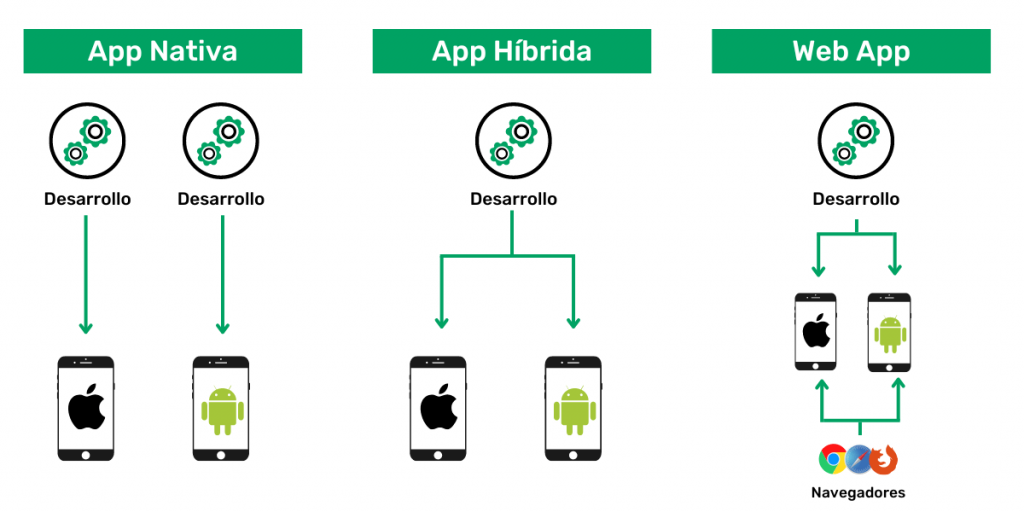
\includegraphics[width=.68\textwidth]{images/img08}}
		\caption{Tipo de aplicaciones moviles \cite{IM1}.}
		\label{fig:casosDeUso}
	\end{center}
\end{figure}

\subsection{Aplicaciones nativas}
Las aplicaciones nativas son apps desarrolladas para un sistema operativo móvil concreto (iOS o Android normalmente), en el lenguaje de programación específico de cada plataforma. Esto quiere decir que una app nativa creada para Android no puede ser utilizada en un dispositivo iOS y viceversa. \\

Es el tipo de aplicación móvil más conocida. Para que funcione, debemos descargarla desde los markets de apps, como App Store o Google Play e instalarla en nuestro teléfono \cite{CitaA02}.

\subsection*{Ventajas}
\begin{itemize}
	\item \textbf{Tienen el mejor rendimiento.} Las aplicaciones nativas son las más rápidas y tienen un rendimiento superior a otros tipos de apps, ya que han sido optimizadas específicamente para el hardware y el sistema operativo del dispositivo.
	\item \textbf{Acceso completo e integración con las funciones hardware del dispositivo.} Las apps nativas permiten aprovechar al máximo las funcionalidades móviles: cámara, micrófono, lector biométrico de huella, sensores y redes inalámbricas.
	\item \textbf{Pueden funcionar sin acceso a internet (funcionamiento offline)} si han sido diseñadas para ello.
\end{itemize}

\subsection*{Desventajas}
\begin{itemize}
	\item \textbf{Costes de desarrollo altos.} Si queremos tener nuestra app disponible para los dos sistemas, necesitaremos dos líneas de desarrollo diferentes, ya que el código utilizado para un sistema no es reutilizable para otro.
	\item \textbf{Complejidad de desarrollo.} Necesitamos equipos expertos en el lenguaje específico de cada sistema. Por ejemplo, en Kotlin para Android y en Swift para iOS.
	\item \textbf{Tiempo de desarrollo superior.} El desarrollo puede tomar entre 4 a 6 meses.
\end{itemize}

\subsection{Aplicaciones Web}

Las aplicaciones web realmente son webs especiales diseñadas para navegadores móviles. A diferencia de las apps nativas o híbridas, no necesitan ser descargadas, ya que se accede a ellas desde un navegador web.

Emplean las mismas tecnologías de desarrollo que una web, como HTML, CSS o JavaScript. Así, estaríamos hablando de una web con apariencia de app, por lo que presentaría sus mismas limitaciones. Sin embargo, con la llegada del HTML5, se han conseguido salvar algunas limitaciones, como el acceso a algunas funciones del móvil (geolocalización, cámaras) \cite{IM1}.

\subsection*{Ventajas}
\begin{itemize}
	\item \textbf{Carácter multiplataforma.} Con una sola línea de desarrollo.
	\item \textbf{Fácil desarrollo.} Se emplean tecnologías ampliamente conocidas.
	\item \textbf{Tiempo y coste de desarrollo bajo.}
\end{itemize}

\subsection*{Desventajas}
\begin{itemize}
	\item \textbf{Acceso limitado a las funciones del dispositivo.}
	\item \textbf{No se pueden subir a las tiendas de aplicaciones.}
	\item \textbf{Diferentes experiencias de usuario.} Estas dependen del navegador utilizado.
	\item \textbf{Necesidad de conexión a Internet.} Incluso si se cuenta con un modo pensado para ello, es necesario para acceder a las posibles actualizaciones o para entrar por primera vez.
\end{itemize}

\subsection{Aplicaciones Híbridas}

Las aplicaciones híbridas o multiplataforma combinan elementos de las aplicaciones nativas y las aplicaciones web. Estas aplicaciones se desarrollan utilizando tecnologías web como HTML, CSS y JavaScript, pero se empaquetan en un formato que puede ser instalado en un dispositivo móvil como cualquier otra aplicación nativa. Por tanto, podemos obtener una aplicación para varias plataformas con un único desarrollo \cite{IM1}.

\subsection*{Ventajas}
\begin{itemize}
	\item \textbf{Menor coste.} Gracias al uso de lenguajes de programación más conocidos, con una mayor disponibilidad de profesionales en el mercado.
	\item \textbf{Carácter multiplataforma.} Con una sola línea de desarrollo.
	\item \textbf{Acceso a algunas funcionalidades del móvil.}
	\item \textbf{Reducción de los tiempos de desarrollo.} Generalmente, el tiempo de desarrollo se reduce a 3 meses.
	\item \textbf{Disponibilidad en markets.} Se pueden subir a los markets de aplicaciones, como App Store y Google Play.
\end{itemize}

\subsection*{Desventajas}
\begin{itemize}
	\item \textbf{Rendimiento inferior.} Su rendimiento es inferior al de una app nativa, suelen tener un tamaño considerable y, además, ser más lentas.
	\item \textbf{Acceso limitado a las funciones del dispositivo.}
\end{itemize}

\subsection{Aplicaciones Progresivas Web Apps (PWA)}

Las aplicaciones progresivas son un reciente avance de las Web Apps. Al igual que las Web Apps, son webs diseñadas para móviles, pero esta vez, sí pueden ser descargadas en el móvil como una aplicación más, aunque no es necesario para que ofrezcan un comportamiento similar al de una app nativa a través del navegador. \\

Las PWA adoptan un comportamiento más propio de aplicaciones nativas que de web, como el funcionamiento sin Internet, un mayor rendimiento o su funcionamiento en segundo plano. Sin embargo, como desventaja, seguimos contando con la imposibilidad de subirlas a los markets de aplicaciones \cite{IM1}. \\

Para comprender mejor las diferencias entre los tipos de aplicaciones móviles, a continuación se presenta una tabla comparativa que destaca sus características clave:
\newpage

\begin{table}[h!]
	\centering
	\begin{tabular}{|p{4cm}|p{2cm}|p{2cm}|p{2cm}|}
		\hline
		\textbf{Tipos de app} & \textbf{Nativa} & \textbf{Híbrida} & \textbf{Web} \\ \hline
		\textbf{Interfaz} & Basada en web & Específica de la plataforma (iOS, Android) & Basada en web \\ \hline
		\textbf{Tiempo de desarrollo} & Alto & Medio & Bajo \\ \hline
		\textbf{Coste de desarrollo} & Alto & Medio & Bajo \\ \hline
		\textbf{Multiplataforma} & No & Sí & Sí \\ \hline
		\textbf{Rendimiento} & Alto & Medio & Bajo \\ \hline
		\textbf{Acceso a los sensores del dispositivo} & Completo & Alto o Completo & Limitado \\ \hline
		\textbf{Tiendas de aplicaciones} & Sí & Sí & No \\ \hline
	\end{tabular}
	\caption{Comparación tipos de aplicaciones móviles. Elaboración propia}
	\label{tab:tipos_apps}
\end{table}

Para el desarrollo de nuestro trabajo terminal, hemos decidido optar por una aplicación híbrida con el uso de Kotlin. Esta decisión se basa en varios factores relacionados con los recursos disponibles, las características de nuestro público objetivo y los plazos establecidos. \\

La aplicación móvil está dirigida para estudiantes, alumnos y personal de seguridad de la Escuela Superior de Cómputo, donde la mayoría utiliza dispositivos con sistema operativo Android. La elección de una aplicación híbrida nos permite optimizar  la experiencia en Android, que es la plataforma que predomina entre nuestros usuarios. \\

Aunque las aplicaciones híbridas suelen desarrollarse con tecnologías web (como React Native o Flutter), para nuestro proyecto hemos decidido incorporar Kotlin para desarrollar modelos donde se requiera un rendimiento nativo o un acceso más profundo a las funciones del sistema operativo Android.Además, las aplicaciones híbridas permiten un desarrollo más rápido en comparación con las aplicaciones completamente nativas, ya que gran parte del código puede compartirse entre plataformas, así mismo, es una buena opción económica que se adapta a nuestro presupuesto \cite{IM1}. 
%---------------------------------------------------------
% !TeX root = ../ejemplo.tex

\section{Elección de tecnología}
La elección de Kotlin como lenguaje principal y Android como plataforma se basa en criterios técnicos, prácticos y económicos que se alinean directamente con los requisitos del proyecto.

\subsection{Kotlin}
Kotlin es un lenguaje de alto nivel debido a su abstracción respecto al hardware y la plataforma subyacente. Esto significa que permite a los desarrolladores escribir código sin preocuparse por la gestión de memoria o las interacciones directas con el sistema operativo o el hardware, lo que mejora la productividad y la legibilidad del código, además, este es estáticamente tipado, lo que implica que los tipos de las variables se definen en tiempo de compilación, lo que permite detectar errores antes de ejecutar el programa. Este se usa principalmente en el desarrollo de aplicaciones Android, donde es el lenguaje recomendado por Google \cite{CitaD14}.

Además, Kotlin permite el uso de Jetpack Compose, un framework declarativo que moderniza la creación de interfaces de usuario en Android. También es compatible con bibliotecas clave para este proyecto como OpenCV, empleada en el módulo de reconocimiento facial.

\subsection{Android}
La decisión de desarrollar exclusivamente para Android se basa en:

\begin{itemize}
	\item La mayoría de los usuarios objetivo (alumnos, docentes y personal de seguridad) utilizan dispositivos Android.
	
	\item Android permite mayor flexibilidad y personalización, crucial para funciones como escaneo de códigos QR, acceso a la cámara, integración con Python y OpenCV.
	
	\item El entorno Android es ideal para pruebas, ya que se puede emular fácilmente en computadoras con Windows.
\end{itemize}

La compatibilidad de Android con Python facilita la integración del frontend (Android) con el backend, donde Python se encarga del procesamiento de imágenes y entrenamiento de modelos de reconocimiento facial, mientras que Spring Boot gestiona la lógica del sistema. Esta arquitectura garantiza un funcionamiento sincronizado, eficiente y seguro.


\section{Herramientas de Desarrollo}
El desarrollo de la aplicación se realizó con herramientas modernas que forman parte del ecosistema oficial de Android, permitiendo una implementación robusta y escalable.

\subsection{Android Studio}
Android Studio es el entorno de desarrollo integrado (IDE) oficial para el desarrollo de aplicaciones del mismo OS. Se basa en IntelliJ IDEA, un entorno de desarrollo integrado de Java para software, e incorpora sus herramientas de desarrollo y edición de código \cite{CitaD19}.

Para respaldar el desarrollo de aplicaciones dentro del sistema operativo, Android Studio utiliza un sistema de compilación basado en Gradle, un emulador de Android, plantillas de código e integración de GitHub. Cada proyecto en Android Studio tiene una o más modalidades con código fuente y archivos de recursos \cite{CitaD19}.

\subsection{Jetpack Compose}
Para la implementación de la aplicación móvil que forma parte de nuestro sistema de identificación y control de acceso, hemos decidido utilizar Jetpack Compose. La elección de la tecnología adecuada es importante para ofrecer una mejor experiencia de usuario y cumplir nuestros objetivos de diseño y funcional. 

\subsection*{¿Por que Jetpack compose?}
Jetpack compose es un framework (estructura o marco de trabajo que, bajo parámetros estandarizados, ejecutan tareas específicas en el desarrollo de un software) con la particularidad de ejecutar prácticas modernas en los desarrolladores de software a partir de la reutilización de componentes, así como también contando con la oportunidad de crear animaciones y temas oscuros. En este sentido, Jetpack Compose es el conjunto de herramientas ofrecidas por Android para el desarrollo de aplicaciones con un objetivo específico: simplificar y optimizar los códigos en la IU nativas \cite{CitaA01}. 


\subsection*{Ventajas}

\begin{itemize}
	\item \textbf{Menos código:} Simplifica el proceso de desarrollo haciendo menos código, todo se basa en funciones de modo que el código será simple y fácil de mantener.
	\item \textbf{Intuitiva:} Tan solo describe tu IU con un enfoque declarativo haciendo “qué hay que hacer” en vez de “cómo se debe hacer”.
	\item \textbf{Potente:} Tiene integrado Material Design con el cual puede crear apps atractivas al usuario con animaciones y mucho más.
	\item \textbf{Acelera el desarrollo:} Es compatible con proyectos existentes, puedes empezar a integrarlo por partes cuando quieras y donde quieras.
	\item \textbf{Kotlin:} Está escrito 100\% en Kotlin, lo cual nos permitirá usar sus herramientas potentes y API’s intuitivas.
\end{itemize}

\subsection*{Arquitectura Jetpack}
La arquitectura o estructura sobre la que se basa Jetpack Compose es una estructura Jetpack que se encarga principalmente de seguir ejecutando y beneficiándose de aquellos componentes de Android según la funcionalidad disponible. Por lo tanto, Jetpack Compose desarrolla herramientas denominadas «composables» a partir de elementos como botones o listados de objetos. A partir de fuentes de datos, pueden ser reutilizadas y ejecutadas en distintas fuentes sin la necesidad de programar varios códigos repetitivos.

Desde un aspecto comparativo, la creación de UI con Compose se realiza de forma similar a los de React Native. Es decir, mediante componentes reutilizables evitan maximizar la cantidad de códigos necesarios y repetitivos, tal como ocurre con HTML en la forma en la que se conjugan uno con otro. Sin embargo, es importante destacar que dicha compilación de componentes que logran la disminución en cantidad de códigos se realiza gracias a los plugins de compiladores de Kotlin, ejecutando así los componentes mediante la estructura de archivos de Kotlin \cite{CitaA19}. 

\subsection*{Estructura de Jetpack Compose}
Para entender de forma más sencilla la estructura de esta herramienta, conviene tener en cuenta componentes como:
\begin{itemize}
	\item \textbf{Compiler:} Se encarga mediante una estructura de plugins en Gradle, donde logra la interpretación y simplificación de códigos.
	\item \textbf{El entorno de ejecución:} Es el ámbito “depurador”, si se puede establecer de este modo, en el que se establecen y diferencian los componentes que necesitan actualización y cuáles no, así como también se crean listados de mantenimiento y composición.
	\item \textbf{UI:} Es el componente que interpreta el lenguaje establecido en el entorno de ejecución y lo refleja en pantalla.
\end{itemize}

\subsection{Gradle}

\begin{list}{}%
	{\setlength{\leftmargin}{1cm}\setlength{\rightmargin}{1cm}}
	\item\relax
	\small
	
	Gradle es el sistema de automatización de compilación utilizado por Android Studio, y fue esencial para el desarrollo del presente proyecto, permitiendo una integración fluida entre los módulos móviles y el backend. Esta herramienta de código abierto destaca por su rendimiento y flexibilidad, utilizando Kotlin DSL (Domain Specific Language) para definir scripts de compilación \cite{CitaD20}. 
	
	Gradle facilita la gestión eficiente de dependencias externas como Jetpack Compose, Retrofit y OpenCV, utilizadas en el desarrollo de la aplicación. Además, su capacidad para realizar compilaciones optimizadas en paralelo y reutilizar salidas anteriores permite reducir considerablemente los tiempos de construcción. También permite configurar distintos entornos de ejecución (debug y release), lo que fue útil para probar características específicas antes de su despliegue oficial. 
	
	En este proyecto, Gradle también permitió la integración con servicios backend mediante llamadas a APIs REST, conectando la aplicación con el servidor desarrollado en Spring Boot, fortaleciendo así la arquitectura cliente-servidor de la solución.
	
\end{list}

\subsection{Git y GitHub}

\begin{list}{}%
	{\setlength{\leftmargin}{1cm}\setlength{\rightmargin}{1cm}}
	\item\relax
	\small
	
	Durante el desarrollo del proyecto, se utilizó Git como sistema de control de versiones y GitHub como plataforma de colaboración y almacenamiento en la nube. Git, diseñado por Linus Torvalds, permite llevar un control detallado del historial de cambios en el código, lo cual es esencial en proyectos donde trabajan varios desarrolladores de forma simultánea \cite{CitaD20}.
	
	Cada miembro del equipo pudo trabajar en ramas independientes, realizar modificaciones, proponer mejoras y fusionar los cambios mediante revisiones de código, garantizando la integridad del repositorio principal. Esta metodología permitió detectar errores, revertir versiones cuando fue necesario, y mantener una trazabilidad clara del desarrollo de cada módulo.
	
	GitHub, además de servir como repositorio central, funcionó como herramienta de comunicación y documentación del avance del proyecto. Las funcionalidades de issues, pull requests y proyectos ayudaron a distribuir tareas, dar seguimiento a problemas y mantener una organización clara durante todo el ciclo de desarrollo \cite{CitaD21}.
	
\end{list}



%---------------------------------------------------------
% !TeX root = ../ejemplo.tex

\section{Lenguaje de programación}

Una vez establecido el sistema operativo que vamos a usar, nos interesa establecer que es un lenguaje de programación.
\begin{list}{}%
    {\setlength{\leftmargin}{1cm}\setlength{\rightmargin}{1cm}}
    \item\relax
    \small
En términos generales, un lenguaje de programación es una herramienta que permite desarrollar software o programas para computadora. Los lenguajes de programación son empleados para diseñar e implementar programas encargados de definir y administrar el comportamiento de los dispositivos físicos y lógicos de una computadora. Lo anterior se logra mediante la creación e implementación de algoritmos de precisión que se utilizan como una forma de comunicación humana con la computadora \cite{CitaD10}.

A grandes rasgos, un lenguaje de programación se conforma de una serie de símbolos y reglas de sintaxis y semántica que definen la estructura principal del lenguaje y le dan un significado a sus elementos y expresiones \cite{CitaD10}.
\end{list}
Estos se dividen en 3 tipos: lenguajes máquina, lenguajes de bajo nivel y lenguajes de alto nivel.


\subsection{Lenguajes máquina}

\begin{list}{}%
    {\setlength{\leftmargin}{1cm}\setlength{\rightmargin}{1cm}}
    \item\relax
    \small

Es el sistema de códigos interpretable directamente por un circuito microprogramable, como el microprocesador de una computadora. Este lenguaje se compone de un conjunto de instrucciones que determinan acciones que serán realizadas por la máquina. Y un programa de computadora consiste en una cadena de estas instrucciones de lenguaje de máquina (más los datos). Normalmente estas instrucciones son ejecutadas en secuencia, con eventuales cambios de flujo causados por el propio programa o eventos externos. El lenguaje máquina es específico de cada máquina o arquitectura de la máquina, aunque el conjunto de instrucciones disponibles pueda ser similar entre ellas \cite{CitaD10}.

\end{list}

\subsection{Lenguajes de alto nivel}

\begin{list}{}%
    {\setlength{\leftmargin}{1cm}\setlength{\rightmargin}{1cm}}
    \item\relax
    \small

Un lenguaje de programación de bajo nivel es el que proporciona poca o ninguna abstracción del microprocesador de una computadora. Consecuentemente, su trasladado al lenguaje máquina es fácil. El término ensamblador (del inglés assembler) se refiere a un tipo de programa informático encargado de traducir un archivo fuente, escrito en un lenguaje ensamblador, a un archivo objeto que contiene código máquina ejecutable directamente por la máquina para la que se ha generado \cite{CitaD10}. 

\end{list}

\subsection{Lenguajes de bajo nivel}

\begin{list}{}%
    {\setlength{\leftmargin}{1cm}\setlength{\rightmargin}{1cm}}
    \item\relax
    \small

Los lenguajes de programación de alto nivel se caracterizan porque su estructura semántica es muy similar a la forma como escriben los humanos, lo que permite codificar los algoritmos de manera más natural, en lugar de codificarlos en el lenguaje binario de las máquinas, o a nivel de lenguaje ensamblador \cite{CitaD10}. 

\end{list}

Entre estos tipos de lenguajes nos interesa los lenguajes de alto nivel ya que para el proyecto estamos considerando el uso de Python, Java y Kotlin, que son considerados lenguajes de alto nivel. Concretamente Python es un lenguaje multiparadigma que puede ser estructurado como si se usara la programación orientada a objetos, Java usa la programación orientada a objetos y Kotlin puede trabajar con esta orientación por lo que antes de definir qué son estos dos lenguajes es de vital importancia definir qué es la “programación orientada a objetos”.


\subsection{Programación orientada a objetos}

\begin{list}{}%
    {\setlength{\leftmargin}{1cm}\setlength{\rightmargin}{1cm}}
    \item\relax
    \small

La programación orientada a objetos (POO) es un modelo de programación informática que organiza el diseño del software en torno a datos u objetos, en lugar de funciones y lógica. Un objeto puede definirse como un campo de datos que tiene unos atributos y comportamientos únicos\cite{CitaD11}.
Los ejemplos de un objeto pueden ir desde entidades físicas, como un ser humano que se describe por propiedades como el nombre y la dirección, hasta pequeños programas informáticos, como los widgets\cite{CitaD11}.
La POO se centra en los objetos que los desarrolladores quieren manejar, en lugar de la lógica necesaria para hacerlo. Este enfoque de la programación es muy adecuado para programas grandes, complejos y que se actualizan o mantienen activamente\cite{CitaD11}.
Esto incluye programas para la producción y el diseño web, así como aplicaciones móviles\cite{CitaD11}.

\end{list}

\subsection{Python}

\begin{list}{}%
    {\setlength{\leftmargin}{1cm}\setlength{\rightmargin}{1cm}}
    \item\relax
    \small

En términos técnicos, Python es un lenguaje de programación de alto nivel, orientado a objetos, con una semántica dinámica integrada, principalmente para el desarrollo web y de aplicaciones informáticas, o a nivel de lenguaje ensamblador\cite{CitaD12}.
Python es relativamente simple, por lo que es fácil de aprender, ya que requiere una sintaxis única que se centra en la legibilidad. Los desarrolladores pueden leer y traducir el código Python mucho más fácilmente que otros lenguajes\cite{CitaD12}.
Por tanto, esto reduce el costo de mantenimiento y de desarrollo del programa porque permite que los equipos trabajen en colaboración sin barreras significativas de lenguaje y experimentación\cite{CitaD12}.
Además, soporta el uso de módulos y paquetes, lo que significa que los programas pueden ser diseñados en un estilo modular y el código puede ser reutilizado en varios proyectos. Una vez se ha desarrollado un módulo o paquete, se puede escalar para su uso en otros proyectos, y es fácil de importar o exportar\cite{CitaD12}.
Por otro lado, uno de los beneficios más importantes de Python es que tanto la librería estándar como el intérprete están disponibles gratuitamente, tanto en forma binaria como en forma de fuente\cite{CitaD12}.
Tampoco hay exclusividad, ya que Python y todas las herramientas necesarias están disponibles en todas las plataformas principales \cite{CitaD12}.

\end{list}


\subsection{Java}

\begin{list}{}%
    {\setlength{\leftmargin}{1cm}\setlength{\rightmargin}{1cm}}
    \item\relax
    \small

Java es un lenguaje orientado a objetos; es decir que organiza el trabajo en torno a objetos en lugar de funciones y lógica. Las aplicaciones móviles y herramientas de software, incluidos los mundialmente famosos Amazon, Spotify y Minecraft, se basan en Java.
Java tiene dos propiedades que determinan qué tareas se pueden resolver con él.
Java es un lenguaje de programación orientado a objetos (POO). Toda interacción en él se produce a través de objetos. Estas entidades se describen en código y se les enseña a interactuar entre sí. Como resultado, un programa de estilo orientado a objetos consta de bloques separados que son fácilmente extensibles y escalables. \cite{CitaD13}

\end{list}

Y java tiene la capacidad de interpretar y compilar, es decir tiene un intérprete que se dedica a leer cada línea de código una por una y ejecutarla sin traducirla a lenguaje máquina y además puede transformar su código  a lenguaje máquina y hacer que el procesador lo compile traducido \cite{CitaD13}. 


\subsection{Kotlin}

Kotlin es un lenguaje de alto nivel debido a su abstracción respecto al hardware y la plataforma subyacente. Esto significa que permite a los desarrolladores escribir código sin preocuparse por la gestión de memoria o las interacciones directas con el sistema operativo o el hardware, lo que mejora la productividad y la legibilidad del código, además, este es estáticamente tipado, lo que implica que los tipos de las variables se definen en tiempo de compilación, lo que permite detectar errores antes de ejecutar el programa. Este se usa principalmente en el desarrollo de aplicaciones Android, donde es el lenguaje recomendado por Google \cite{CitaD14}.

Con la información anterior se puede explicar porque consideramos estos tres lenguajes de programación; Primero estos tres lenguajes poseen una misma orientación lo cual nos ayuda a que el desarrollo del proyecto sea más conciso y fácil, después estos son lenguajes de alto nivel que tienen una buena legibilidad lo que le permite al equipo entender de manera más sencilla el trabajo de los demás integrantes, también pueden ser conectados entre ellos de manera relativamente fácil y sobretodo su alta cantidad de bibliotecas de apoyo y su características de ser  estándares de desarrollo; en android (Kotlin), de desarrollo para servidores (Python) y Java para desarrollo web.
Otra razón por la que decidimos usar estos tres lenguajes de programación es por su compatibilidad con la API OpenCV la cual será una herramienta clave para el desarrollo de nuestro proyecto, por lo que es necesario explicar que es una API y qué es OpenCV.

%---------------------------------------------------------
% !TeX root = ../ejemplo.tex

\section{API}

\begin{list}{}%
    {\setlength{\leftmargin}{1cm}\setlength{\rightmargin}{1cm}}
    \item\relax
    \small

Una API, o interfaz de programación de aplicaciones, es un conjunto de reglas o protocolos que permiten que las aplicaciones de software se comuniquen entre sí para intercambiar datos, características y funcionalidades \cite{CitaD15}.
Las API simplifican y aceleran el desarrollo de software y aplicaciones permitiendo a los desarrolladores integrar datos, servicios y capacidades de otras aplicaciones, en lugar de desarrollarlas desde cero. Las API también ofrecen a los propietarios de aplicaciones una forma sencilla y segura de poner los datos y las funciones de sus aplicaciones a disposición de los departamentos de su organización. Los propietarios de aplicaciones también pueden compartir o comercializar datos y funciones con asociados de negocios o terceros [24].

\end{list}

\subsection{OpenCV}

\begin{list}{}%
    {\setlength{\leftmargin}{1cm}\setlength{\rightmargin}{1cm}}
    \item\relax
    \small

OpenCV, o Open Source Computer Vision Library, es una colección de más de 2500 algoritmos optimizados que facilitan el procesamiento de imágenes y la realización de diversas operaciones de vision computacional. Fundada por Intel en 2000 y con colaboración de múltiples empresas y desarrolladores, esta biblioteca es de fácil acceso y cuenta con una licencia BSD [25].
Siendo compatible con varios lenguajes de programación, incluido Python, Java y C++, OpenCV permite trabajar en múltiples plataformas y sistemas operativos. Esta biblioteca también destaca por su papel en el impulso de tecnologías emergentes como el deep learning \cite{CitaD16}.

\end{list}

Por último esta cuenta con muchos procesos y funciones que apoyan al reconocimiento facial, además de ser compatible con Python, Kotlin y Java y poseer una alta cantidad de tutoriales que rondan desde las integraciones básicas hasta procesos avanzados.

\subsection{Licencia BSD}

\begin{list}{}%
    {\setlength{\leftmargin}{1cm}\setlength{\rightmargin}{1cm}}
    \item\relax
    \small

"La licencia BSD, también conocida como licencia de distribución de software de Berkeley, es una popular licencia de código abierto que permite el libre uso, modificación y distribución de software \cite{CitaD17}."

\end{list}

Esta licencia nos permite hacer uso de la biblioteca OpenCV de manera libre, lo cual implica que se puede implementar la biblioteca y darle uso al software de manera comercial, nos permite modificar y distribuir el software sin restricciones significativas y nos permite no publicar el código fuente si así lo deseamos.

Ya con el sistema operativo y los lenguajes de programación establecidos, tenemos que especificar las herramientas que nos permitirán escribir, depurar y gestionar el código de manera eficiente. Estas herramientas son los entornos de desarrollo Integrados (IDE, por sus siglas en inglés), que proporcionan un conjunto de funciones como editores de código, depuradores, y compiladores.


%---------------------------------------------------------
% !TeX root = ../ejemplo.tex

\section{IDE}

Un entorno de desarrollo integrado (IDE) es un sistema de software para el diseño de aplicaciones que combina herramientas del desarrollador comunes en una sola interfaz gráfica de usuario (GUI). Generalmente, un IDE cuenta con las siguientes características \cite{CitaD18}:

\begin{list}{}%
    {\setlength{\leftmargin}{1cm}%
     \setlength{\rightmargin}{1cm}%
     \setlength{\itemsep}{0.5\baselineskip}%
     \setlength{\parsep}{0pt}}
     
    \item\relax
    \small
    \textbf{Editor de código fuente:} editor de texto que ayuda a escribir el código de software con funciones como el resaltado de la sintaxis con indicaciones visuales, el relleno automático específico para el lenguaje y la comprobación de errores a medida que se escribe el código \cite{CitaD18}.
    \textbf{Automatización de las compilaciones locales:} herramientas que automatizan las tareas sencillas y repetitivas como parte de la creación de una compilación local del software para que use el desarrollador, como la compilación del código fuente de la computadora en código binario, el empaquetado de ese código y la ejecución de pruebas automatizadas \cite{CitaD18}.
    \textbf{Depurador:} programa que sirve para probar otros programas y mostrar la ubicación de un error en el código original de forma gráfica \cite{CitaD18}.

\end{list}

Para nuestro proyecto ocuparemos el IDE llamado android studio.

\subsection{Android Studio}

\begin{list}{}%
    {\setlength{\leftmargin}{1cm}\setlength{\rightmargin}{1cm}}
    \item\relax
    \small

Android Studio es el entorno de desarrollo integrado (IDE) oficial para el desarrollo de aplicaciones del mismo OS. Se basa en IntelliJ IDEA, un entorno de desarrollo integrado de Java para software, e incorpora sus herramientas de desarrollo y edición de código \cite{CitaD19}.

Para respaldar el desarrollo de aplicaciones dentro del sistema operativo, Android Studio utiliza un sistema de compilación basado en Gradle, un emulador de Android, plantillas de código e integración de GitHub. Cada proyecto en Android Studio tiene una o más modalidades con código fuente y archivos de recursos \cite{CitaD19}.

\end{list}


\subsection{Gradle}

\begin{list}{}%
    {\setlength{\leftmargin}{1cm}\setlength{\rightmargin}{1cm}}
    \item\relax
    \small

Gradle, es una herramienta que permite la automatización de compilación de código abierto, la cual se encuentra centrada en la flexibilidad y el rendimiento. Los scripts de compilación de Gradle se escriben utilizando Kotlin DSL (Domain Specific Language) \cite{CitaD20}.
Gradle tiene una gran flexibilidad y nos deja hacer usos de otros lenguajes y no solo de Java, también cuenta con un sistema de gestión de dependencias muy estable. Gradle es altamente personalizable y rápido ya que completa las tareas de forma rápida y precisa reutilizando las salidas de las ejecuciones anteriores, sólo procesar las entradas que presentan cambios en paralelo \cite{CitaD20}.
Además es el sistema de compilación oficial para Android y cuenta con soporte para diversas tecnologías y lenguajes \cite{CitaD20}.

\end{list}


\subsection{GitHub}

\begin{list}{}%
    {\setlength{\leftmargin}{1cm}\setlength{\rightmargin}{1cm}}
    \item\relax
    \small

GitHub es una plataforma de desarrollo colaborativo que aloja proyectos en la nube utilizando el sistema de control de versiones llamado Git. Ayuda a los desarrolladores a almacenar y administrar el código llevando un registro de cambios. Generalmente el código es abierto, lo que permite realizar proyectos compartidos y mantener el seguimiento detallado de su progreso. La plataforma GitHub también funciona como red social conectando a los desarrolladores con los usuarios. Como usuario puedes descargar programas o aplicaciones, y de la misma manera puedes aportar a su desarrollo ofreciendo mejoras y discutir las cuestiones que te interesan en foros temáticos \cite{CitaD21}.
\end{list}

\subsection{Git}

\begin{list}{}%
    {\setlength{\leftmargin}{1cm}\setlength{\rightmargin}{1cm}}
    \item\relax
    \small

Git es un software de control de versiones diseñado por Linus Torvalds, el creador de Linux. El propósito de Git es llevar un registro de cambios y coordinar el trabajo de varias personas en un repositorio compartido. Desde su creación en 2005, este software llegó a convertirse en uno de los VCS más populares: según la encuesta de Stack Overflow (en inglés), más del noventa porciento de los desarrolladores usan Git en sus proyectos \cite{CitaD20}.
Git proporciona herramientas para un trabajo rápido y eficiente dentro de un equipo. El control de versiones permite a los desarrolladores descargar una copia del código fuente a sus repositorios locales (PC), realizar cambios y subir una versión nueva al repositorio compartido. Todas las modificaciones se guardan en versiones independientes, sin afectar el archivo original. Se pueden comparar cambios realizados, ver quién modificó el código y determinar en qué momento se introdujo un error para poder revertirlo. De esta forma todos los desarrolladores interesados en el proyecto tienen acceso al historial de modificaciones realizadas y pueden contribuir mejorando el código del software \cite{CitaD21}.

\end{list}

Esta última es una herramienta que tenemos planeada usar para el control de versiones en nuestro proyecto. 

%---------------------------------------------------------
% !TeX root = ../ejemplo.tex

\section{Framework}
\subsection{Jetpack compose}
Para la implementación de la aplicación móvil que forma parte de nuestro sistema de identificación y control de acceso, hemos decidido utilizar Jetpack Compose. La elección de la tecnología adecuada es importante para ofrecer una mejor experiencia de usuario y cumplir nuestros objetivos de diseño y funcional. 

\subsection*{¿Por que Jetpack compose?}
Jetpack compose es un framework (estructura o marco de trabajo que, bajo parámetros estandarizados, ejecutan tareas específicas en el desarrollo de un software) con la particularidad de ejecutar prácticas modernas en los desarrolladores de software a partir de la reutilización de componentes, así como también contando con la oportunidad de crear animaciones y temas oscuros. En este sentido, Jetpack Compose es el conjunto de herramientas ofrecidas por Android para el desarrollo de aplicaciones con un objetivo específico: simplificar y optimizar los códigos en la IU nativas \cite{CitaA01}. 


\subsection*{Ventajas}

\begin{itemize}
	\item \textbf{Menos código:} Simplifica el proceso de desarrollo haciendo menos código, todo se basa en funciones de modo que el código será simple y fácil de mantener.
	\item \textbf{Intuitiva:} Tan solo describe tu IU con un enfoque declarativo haciendo “qué hay que hacer” en vez de “cómo se debe hacer”.
	\item \textbf{Potente:} Tiene integrado Material Design con el cual puede crear apps atractivas al usuario con animaciones y mucho más.
	\item \textbf{Acelera el desarrollo:} Es compatible con proyectos existentes, puedes empezar a integrarlo por partes cuando quieras y donde quieras.
	\item \textbf{Kotlin:} Está escrito 100\% en Kotlin, lo cual nos permitirá usar sus herramientas potentes y API’s intuitivas.
\end{itemize}
%---------------------------------------------------------
% !TeX root = ../ejemplo.tex

\section{Bases de datos (BD)}
Para que todo sistema pueda funcionar, debe de tener una forma de almacenar toda su información, ya sea información de los usuarios o para almacenar imágenes, cualquier tipo de información que se requiera almacenar, es necesario usar una base de datos. Pero en sí, ¿qué es una base de datos?.
Una base de datos, según Microsoft \cite{CitaAJ08} , es una herramienta para recopilar y organizar información. Estas pueden almacenar información sobre personas, productos, pedidos u otras cosas. Las bases de datos pueden empezar desde un simple documento de textos o archivos Excel, pero conforme más va creciendo esta base de datos empiezan a aparecer redundancias, por lo que es mejor optar por usar una base de datos creada por un sistema gestor de bases de datos. 
Un sistema gestor de bases de datos es un software constituido por una serie de programas dirigidos a crear, gestionar y administrar la información que se encuentra en una base de datos. El principal objetivo de estos sistemas es servir de interfaz entre los usuarios y las aplicaciones para facilitar la organización de los datos \cite{CitaAJ06}.
Por otro lado, dentro del mundo de las bases de datos, existen diferentes tipos de bases de datos, y cada tipo de base de datos tiene una organización diferente y propósito diferente. A continuación, les hablaremos de ciertos tipos de bases de datos:

\subsection{Bases de datos relacionales:}
Este tipo de bases de datos es el más usado en sistemas que necesitan almacenar una gran cantidad de información que está relacionada entre sí. Ahora bien, una base de datos relacional, según Google \cite{CitaAJ09}, es una forma de estructurar información en tablas, filas y columnas. La ventaja de este tipo de bases de datos es que tiene la capacidad de establecer relaciones entre la información mediante tablas, esto nos ayuda a visualizar mejor la información sobre la relación entre los datos.
Las bases de datos relacionales se componen de una serie de conceptos clave que necesitamos desarrollar para mejorar la comprensibilidad acerca de este tipo de bases de datos:

\begin{itemize}
    \item \textbf{Tablas:} Las tablas, en una base de datos relacional, son objetos que contienen todos los datos de dicho objeto. Como se mencionó anteriormente, estas tablas se organizan en filas y columnas. Aquí, cada fila representa un registro único y cada columna un campo dentro del registro. La manera en que este tipo de tablas guardan datos únicos es por medio de una clave principal, la cuál se va a explicar a continuación. \cite{CitaAJ10}
    \item \textbf{Clave principal:} Como ya se mencionó, las tablas tienen una clave principal, la cuál suele ser una columna o un conjunto de columnas cuyos valores identifican la forma única de cada fila de la tabla. Estas columnas se denominan claves principales de la tabla y aunque la clave principal sea una combinación de columnas, esta combinación es única dentro de la tabla. \cite{CitaAJ11}
    \item \textbf{Clave externa:} Esta es una columna o combinación de columnas que se usa para establecer un vínculo entre los datos de dos tablas. Cuando una tabla tiene dentro de sus columnas la clave principal de otra tabla, se dice que esa primera tabla está referenciando a la otra por medio de una clave externa. \cite{CitaAJ12}
    \item \textbf{Sistema de gestión de bases de datos (SGBD):} Son sistemas que ayudan a controlar las bases de datos. Estos sistemas actúan como interfaz entre los usuarios y las bases de datos, y se encargan justamente de gestionar los datos y las bases de datos como tal. En otras palabras, un sistema de gestión de bases de datos es un software utilizado para gestionar, almacenar y recuperar bases de datos, a su vez, proporciona una interfaz que permite a los usuarios leer, crear, borrar y actualizar datos. \cite{CitaAJ06}
\end{itemize}

\subsubsection{PostgreSQL:}
PostgreSQL es una SGBD relacional, el cual, a diferencia de otros este soporta tipos de datos relacionales y no relacionales. Este fue creado con el propósito de soportar cagras de trabajo desde pequeñas aplicaciones hasta sistemas complejos de procesamiento de datos a gran escala. 
Para este proyecto, se hará uso de este SGBD, ya que tiene compatibilidad con los diferentes lenguajes que vamos a usar, como lo es Java, y además, es libre de restricciones de licencia. \cite{CitaAJ05}

\subsection{Bases de datos no relacionales:}
Este tipo de bases de datos no siguen el esquema de filas y columnas como las bases de datos relacionales, en su lugar, este tipo de bases de datos usan un modelo de almacenamiento que está optimizado para los requisitos del tipo de dato que van a guardar. Dentro de este tipo de bases de datos existe una gran variedad, hay bases de datos que almacenan su información como pares clave/valor simple, como formatos JSON, o como un grafo que consta de bordes y vértices. Lo que caracteriza a este tipo de bases de datos es que no usan el modelo relacional. \cite{CitaAJ12}

%---------------------------------------------------------
% !TeX root = ../ejemplo.tex

\section{Spring Boot}
Spring Boot es una herramienta que sirve para desarrollar tanto aplicaciones web, como microservicios en Java. Este se basa en Spring Framework, el cual es un framework para el desarrollo de aplicaciones y contenedores de inversión de control de código abierto, igualmente para Java.
Spring Boot permite el desarrollo de aplicaciones web y microservicios de manera rápida y fácil gracias a 3 características que tiene, las cuales son:
\begin{itemize}
    \item \textbf{Configuración automática:} Con esto se refiere a que Spring Boot lo que hace es analizar las dependencias incluidas en un proyecto, como lo son bases de datos, servidores, entre otras cosas y decide qué configuraciones aplicar. Esto se basa en anotaciones que usualmente empiezan con un "@", gracias a esto, podemos desarrollar aplicaciones de manera más rápida y eficiente, pues nos ahorra todo el trabajo de realizar método por método. \cite{CitaAJ01}
    \item \textbf{Enfoque obstinado de la configuración:} Con base en las mejores prácticas de la programación, Spring Boot toma ciertas decisiones de configuración que funcionan bien para la mayoría de casos, esto se refiere a configuraciones de puertos, rutas, entre otras cosas. Además, en caso de que nosotros queramos agregar configuraciones adicionales, o bien, cambiar la configuración de algo de nuestro proyecto, nos va a crear un archivo de configuración en donde podremos especificarle de qué manera lo queremos. \cite{CitaAJ02}
    \item \textbf{Capacidad de crear aplicaciones independientes:} Nos permite crear aplicaciones que se ejecutan de forma independiente, es decir, sin necesidad de un servidor web externo. Esto lo logra gracias a que en el proceso de inicialización, se integra un servidor web en la aplicación, o que le permite funcionar de manera autónoma. \cite{CitaAJ01}
\end{itemize}

\section{Java Persistence API (JPA)}
Antes de irnos a la definición de JPA, hay que entender qué es la persistencia de los datos. La persistencia de los datos es un medio mediante el cual una aplicación puede recuperar información desde un sistema de almacenamiento y hacer que esta persista. Ahora bien, JPA lo que hace es proporcionarnos varias funciones para poder gestionar la persistencia y la correlación de objetos, es decir, lo que hace es proveernos con una serie de interfaces que podemos utilizar para implementar la capa de persistencia de nuestra aplicación. \cite{CitaAJ03}

Algunas de las ventajas que nos presenta JPA es que nos permite hacer el mapeo de entidades, es decir, el definir cómo se relacionan las clases de nuestra aplicación con los elementos de nuestra base de \cite{CitaAJ03}. Esto abarca temas como las relaciones entre clases y tablas en nuestra abse de datos, propiedades de las clases y los campos de las tablas e incluso la relación entre diferentes clases y las claves exrternas de nuestras tablas. 

Además, JPA ofrece la capacidad de interactuar con diferentes sistemas de gestión de bases de datos, ya que no usa sentencias SQL o de algún tipo de base de datos en específico, por lo que mejora la portabilidad y escalabilidad de las aplicaciones. \cite{CitaAJ04}
%---------------------------------------------------------
% !TeX root = ../ejemplo.tex

\section{Patrones de arquitectura de software}
Al momento de desarrollar software, es común toparnos con problemáticas que requieren de la toma de decisiones especialmente cuando hablamos sobre cuestiones relacionadas con el diseño de un sistema de software.
Un patrón de arquitectura de software es un conjunto de decisiones tomadas para atacar problemáticas relacionadas con el diseño de un software. Estos incluyen reglas y principios para organizar las interacciones entre subsistemas predefinidos y los roles que estos desempeñan \cite{L07}.

A menudo pueden ser descritos como los \textit{"Planos"} de un sistema, sin embargo, esto no quiere decir que sea la arquitectura final, sino que funcionan como una guía que describe los elementos necesarios para diseñar la arquitectura de la solución a desarrollar, la selección de una arquitectura sobre otra dependerá completamente de los objetivos a alcanzar, los recursos disponibles y la experiencia del equipo de desarrollo \cite{L08}.

Es necesario aclarar que, los patrones de arquitectura no deben confundirse con los patrones de diseño, ya que ambos responden a problemas diferentes durante el desarrollo de un sistema de software, de forma muy breve un patrón de arquitectura describe como crear la lógica de negocio, acceso a los datos, etc. Mientras que los patrones de diseño se usan al implementar estos elementos \cite{L07}.

A continuación, se describen algunos patrones de arquitectura que pueden ser de utilidad al implementar la propuesta de solución para este trabajo terminal.	

\subsection{Arquitectura de capas}

También conocida como \textit{arquitectura de N-capas}, estructura una aplicación en múltiples capas distintas, donde cada una esta encargada de ciertas tareas en especifico, lo que permite dividir un sistema en componentes aislados, lo que facilita el desarrollo rápido de aplicaciones ya que los cambios realizados en una capa no deberían afectar la lógica de las demás \cite{L09}.

Las arquitecturas basadas en este patrón suelen implementar cuatro capas distintas, la capa de presentación, la capa de negocio, de persistencia y de base de datos, sin embargo, y como es de esperarse, la arquitectura de un sistema basado en este patrón puede tener algunas diferencias en el número y tipo de capas que se implementan, por ejemplo, algunas pueden implementar capas de aplicación, servicio o acceso a datos \cite{L07}.

\subsection{Arquitectura orientada a servicios}

Las aplicaciones diseñadas siguiendo este patrón de arquitectura implementan una colección de servicios poco acoplados que se comunican entre sí a través de una red.
Cada uno de los servicios que conforman al sistema se encarga de llevar acabo una función del negocio en específico que después pueden ser requeridos por otro servicio o cliente \cite{L09}.


\subsection{Arquitectura de micro servicios}

Es una arquitectura que combina patrones de diseño para crear múltiples servicios que trabajan de forma independiente y que en conjunto forman la lógica de una aplicación. Es una alternativa a las aplicaciones monolíticas y de la arquitectura basada en servicios, en donde cada servicio esta orientado a implementar partes muy puntuales de la lógica de negocio \cite{L08}.

Su principal ventaja radica en que debido a que sus componentes se encuentran poco acoplados pueden ser desarrollados, desplegados y probados de forma independiente \cite{L09}.

La principal desventaja de este tipo de arquitectura es que puede llegar a ser compleja de implementar ya que requiere de definir la granularidad correcta de los servicios y establecer una comunicación efectiva entre estos \cite{L07}.

\subsection{El patrón modelo vista controlador}

Este patrón divide divide una aplicación en tres componentes interconectados. El modelo, la vista y el controlador. Esta separación permite organizar el código al desacoplar la lógica del negocio, interfaz de usuario y el manejo de las entradas de los usuarios, lo que a su vez promueve la modularidad, mantenibilidad y escalabilidad \cite{L09}. 

El modelo contiene los datos y lógica de negocio de la aplicación. Se encarga de regresar, almacenar y procesar la información.

La vista, también conocida como interfaz de usuario (UI) despliega la información al usuario y responde a las interacciones del usuario.

El controlador funciona como un intermediario entre el modelo y la vista. Se encarga de gestionar las entradas del usuario, actualizar el modelo y la vista para reflejar los cambios realizados en el modelo \cite{L08}.

%---------------------------------------------------------
% !TeX root = ../ejemplo.tex

\section{Redes neuronales artificiales}

Una red neuronal artificial es una técnica para la creación de programas de computación que son capaces de aprender de los datos. Se basa en el conocimiento actual sobre como funciona el cerebro humano. 
Consisten en un conjunto de nodos o neuronas interconectados entre sí que procesan y aprenden de los datos con los que cuentan, lo que permite llevar a cabo tareas como el reconocimiento de patrones y la toma de decisiones en el aprendizaje de máquina \cite{L10}.


\subsection{Estructura de una red neuronal artificial}
Toda red neuronal esta formada por capas de nodos, o neuronas artificiales, una capa de entrada, una o más capas ocultas y una capa de salida. Cada nodo se conecta a los demás y tiene un peso y un umbral determinado.
A continuación se describe el papel que cada una de estas capas en la arquitectura de una red neuronal común \cite{L11}.

\subsubsection{Capa de entrada}
La capa de entrada es responsable de recibir los datos iniciales en forma de vectores. Cada neurona en esta capa corresponde a una característica del conjunto de datos \cite{L12}.

\subsubsection{Capas ocultas}
Las capas ocultas son el núcleo de las RNA y donde ocurre el procesamiento de los datos. Estas capas aplican transformaciones no lineales mediante funciones de activación, como \textit{ReLU}, \textit{sigmoide}, o \textit{tangente hiperbólica}. El número y tamaño de las capas ocultas determinan la capacidad de la red para modelar patrones complejos \cite{L12}.

\subsubsection{Capa de salida}
La capa de salida genera los resultados finales del modelo. Para tareas de clasificación, por ejemplo, esta capa utiliza funciones como \textit{softmax} para proporcionar probabilidades asociadas a cada clase \cite{L12}.

\section{Proceso de aprendizaje}
Como ya se mencionó con anterioridad, una red neuronal es un sistema complejo que busca imitar la forma en la que el cerebro humano aprende \cite.
Este proceso de aprendizaje se realiza en dos fases conocidas como \textit{backpropagation} y \textit{forward propagation} \cite{L12}:


\subsection{Forward propagation}

\begin{itemize}
	\item \textbf{Capa de entrada:} La capa de entrada contiene nodos que representan cada característica del conjunto de datos inicial. Estos nodos reciben y procesan los datos de entrada.  
	\item \textbf{Pesos y conexiones:} Los pesos asignados a cada conexión entre neuronas determinan la influencia de una neurona sobre otra. Durante el entrenamiento, estos valores se actualizan constantemente para optimizar el rendimiento de la red.  
	\item \textbf{Capas ocultas:} Las neuronas en las capas ocultas combinan las entradas recibidas al multiplicarlas por sus respectivos pesos y sumarlas. Posteriormente, aplican una función de activación que introduce no linealidad, lo que permite identificar relaciones complejas en los datos.  
	\item \textbf{Capa de salida:} Este proceso se repite hasta llegar a la capa de salida, donde se genera el resultado final de la red neuronal.
\end{itemize}



\subsection{Backpropagation}

\begin{itemize}
	\item \textbf{Cálculo del error:} La salida generada por la red se compara con los valores esperados utilizando una función de pérdida. Para problemas de regresión, se emplea comúnmente el \textit{Error Cuadrático Medio} (\textit{Mean Squared Error, MSE}), que calcula la diferencia entre las predicciones y los valores reales:  
	$ {MSE} = \frac{1}{n} \sum_{i=1}^{n} (y_i - \hat{y}_i)^2 $
	
	\item \textbf{Optimización por descenso de gradiente:} Para reducir el error, la red emplea el algoritmo de descenso de gradiente. Este ajusta los pesos calculando la derivada de la función de pérdida con respecto a cada peso, guiando los ajustes necesarios para minimizar el error.  
	
	\item \textbf{Ajuste de pesos:} Este proceso de actualización de pesos se realiza en sentido inverso a través de toda la red, lo que permite optimizar las conexiones entre neuronas.  
	
	\item \textbf{Proceso iterativo de entrenamiento:} Durante el entrenamiento, los pasos de propagación hacia adelante, cálculo del error y retropropagación se repiten varias veces con diferentes muestras de datos, permitiendo que la red refine sus parámetros y aprenda patrones específicos.
\end{itemize}


\subsection{Funciones de activación}
Las funciones de activación son fundamentales para introducir no linealidad en el modelo. Ejemplos comunes incluyen la función \textit{ReLU} (Rectified Linear Unit) y la sigmoide. Estas funciones determinan si una neurona se activa, lo que depende del valor ponderado de sus entradas.


\section{Tipos de redes neuronales}

Las redes neuronales pueden clasificarse en distintos tipos, cada uno diseñado para cumplir propósitos específicos. Aunque no se trata de una lista exhaustiva, a continuación se describen algunas de las variantes más comunes y sus casos de uso principales \cite{L11}:


\subsection{Perceptrón} 
El perceptrón es la red neuronal más antigua, desarrollada por Frank Rosenblatt en 1958. Es el precursor de las redes neuronales modernas.  

\subsection{Perceptrón multicapa} 
También conocidas como \textit{feedforward neural networks}, estas redes están formadas por una capa de entrada, una o más capas ocultas y una capa de salida. Aunque frecuentemente se les llama MLPs, técnicamente están compuestas por neuronas sigmoides y no por perceptrones simples, ya que los problemas del mundo real suelen ser no lineales. Estas redes se entrenan alimentándolas con datos y son la base de aplicaciones como visión por computadora, procesamiento de lenguaje natural y otros modelos avanzados.

\subsection{Redes neuronales convolucionales} 
Las redes neuronales convolucionales (\textit{Convolutional Neural Networks}, CNNs) son una variante de las redes de avance directo que se utilizan principalmente en tareas como el reconocimiento de imágenes, el análisis de patrones y la visión por computadora. Estas redes aplican principios del álgebra lineal, en particular la multiplicación de matrices, para identificar patrones dentro de las imágenes.

\subsection{Redes neuronales recurrentes} 
Las redes neuronales recurrentes (\textit{Recurrent Neural Networks}, RNNs) se caracterizan por tener lazos de retroalimentación en su estructura. Estas redes son especialmente útiles para trabajar con datos temporales, donde las predicciones dependen de la información previa. Por ejemplo, se aplican en la predicción de mercados financieros y en la proyección de ventas.


\section{Limitaciones}
Las RNA tienen la capacidad de capturar patrones complejos en grandes volúmenes de datos. Sin embargo, también presentan desafíos como \cite{L13}:

\begin{itemize}
	\item \textbf{Necesidad de datos:} Requieren grandes cantidades de datos etiquetados para entrenarse adecuadamente.
	\item \textbf{Costo computacional:} Su entrenamiento puede ser intensivo en términos de tiempo y recursos computacionales.
	\item \textbf{Interpretabilidad:} Las predicciones de las RNA suelen ser difíciles de interpretar, lo que plantea retos en aplicaciones críticas.
\end{itemize} 


%---------------------------------------------------------
% !TeX root = ../ejemplo.tex

\section{Reconocimiento facial}

El reconocimiento facial es una técnica que permite a las computadoras predecir la identidad de una persona desde una imagen \cite{L14}.

Tiene múltiples aplicaciones en la industria como el desarrollo de sistemas de asistencia, en la salud, sistemas de seguridad, etc \cite{L15}. 

\subsection{Fundamentos del reconocimiento facial}

A menudo, los términos verificación de rostros e identificación de rostros se usan de forma indistinta, sin embargo, aunque ambos comparten el mismo dominio del problema, lo abordan de forma distinta \cite{L16}.

Para entender mejor la diferencia entre ambas tareas y su papel en el desarrollo de un sistema de reconocimiento facial, es que se presentan las técnicas más comunes que lo conforman \cite{L15}.

\subsubsection{Detección de rostros}

En este paso se incluyen algunas estrategias de preprocesamiento que permiten obtener imágenes de buena calidad para los métodos de extracción de características.
Aquí se localiza la región del rostro en una imagen o video y, dependiendo del contexto es posible aplicar técnicas de alineación o cortado de la imagen para aislar los elementos del fondo. Algoritmos como \textit{Viola-Jones} y modelos basados en \textit{Deep Learning}, como \textit{Multi-task Cascaded Convolutional Networks} (MTCNN), son ampliamente utilizados para esta tarea \cite{L16}. 

\subsubsection{Extracción de características}

Una vez que se tiene localizado el rostro se procede a extraer las características de este. En sistemas tradicionales, solían utilizarse descriptores como Histogramas de Gradientes Orientados (\textit{HOG}) o Escalas de Características Invariantes (\textit{SIFT}). Actualmente, los modelos basados en las redes neuronales profundas, especialmente, las redes neuronales convencionales (CNN), como \textit{FaceNet}, generan representaciones compactas conocidas como embeddings, que capturan la información más relevante del rostro \cite{L14}.

\subsubsection{Comparación y verificación}

Los embeddings faciales obtenidos se comparan con una base de datos utilizando medidas de similitud como la distancia coseno o euclidiana. Este paso permite determinar si dos rostros corresponden a la misma persona (verificación) o identificar a una persona entre múltiples registros (identificación) \cite{L14}.


\subsection{Identificación de rostros}

Como ya se mencionó, la identificación de rostros y la verificación de rostros son dos tareas distintas involucradas al momento de implementar un sistema de reconocimiento facial \cite{L14}.

La identificación facial se refiere a la tarea de identificar la identidad de una persona dada una imagen.La imagen se ingresa por un extractor de características para obtener una representación $f$. Luego, esta representación, entra a una red de clasificación para asignar la identidad asociada a la imagen de entrada \cite{L15}.

La identificación de rostros es una tarea de clasificación, por lo que los sistemas de reconocimiento facial basados en esta tarea son entrenados usando la función \textit{softmax} y la pérdida de entropía cruzada [4].

\subsection{Verificación de rostros}

Contrario a la identificación de rostros, la verificación de rostros busca verificar que dos imágenes pertenecen a la misma entidad \cite{L14}. Por lo tanto, en un sistema de reconocimiento facial basado en la verificación de rostros recibe como entrada una imagen $x$ y el identificador del rostro a ser identificado y la salida es una decisión binaria sobre si la imagen $x$ pertenece a la persona con el identificador dado \cite{L15}.

Este enfoque requiere de un proceso de extracción de características de los rostros de las personas que queremos que el sistema verifique y, por lo tanto, almacenar dichas representaciones en una base de datos \cite{L15}.

\subsection{Identificación mediante verificación}
En los sistemas tradicionales de identificación, se entrena un clasificador con $K$ clases para asignar a cada rostro de entrada una identidad específica de entre $K$ personas en la base de datos. Sin embargo, este enfoque presenta limitaciones de escalabilidad, ya que al agregar una nueva persona, es necesario reentrenar completamente el sistema con $K+1$ clases. Esto ocurre porque el clasificador inicial tiene $K$ neuronas, pero para incluir una nueva identidad, se requiere un clasificador con $K+1$ neuronas \cite{L15}.

\vspace{\baselineskip}

Para abordar este problema, un enfoque más eficiente y escalable es utilizar la comparación basada en similitud, propia de los algoritmos de verificación. En este caso, dado un rostro de entrada $x$, se ejecuta el algoritmo de verificación $K$ veces, una para cada rostro almacenado en la base de datos. La identidad del rostro de entrada se asigna a la correspondiente al ID para el cual el algoritmo de verificación indica una coincidencia \cite{L15}.

Por lo tanto, la ventaja de este tipo de enfoque híbrido radica en el hecho de que es posible agregar nuevas entidades al sistema sin la necesidad de re-entrenar los modelos de deep learning utilizados para la generación de los vectores de características de los rostros, más aún si se combina con algún tipo de mecanismo de almacenamiento de estos como las bases de datos vectoriales para acelerar el proceso de inferencia \cite{L17}.







